% **************************************************************************************************
% ** SPSC Report and Thesis Template
% **************************************************************************************************
%
% ***** Authors *****
% Daniel Arnitz, Paul Meissner, Stefan Petrik
% Signal Processing and Speech Communication Laboratory (SPSC)
% Graz University of Technology (TU Graz), Austria
%
% ***** Changelog *****
% 0.1   2010-08-09   added \remc and \remq commands, \nxtpar now uses \med- instead of \bigskip
%                    replaced \lastfootnotemark by \oldfootnotemark (generalization),
%                    added \chapternote, set \openingquote to 0.4\textwidth, modified \MAttention,
%                    \xspace for marginpar commands, modified \MDanger and \MQuestion
% 0.2   2010-10-03   added \exp, colors "bk*"
% 0.3   2010-11-16   added \twofigs and \twofigsf
% 0.4   2010-12      added \F (Fourier), \ceil and \floor
% 0.5   2011-01      added chapter/section/figure/table/part reference commands, textrel
% 0.6   2011-03      added \avg, modified bkred, bkgreen, and bkblue colors,
%                    added \medskip to \chapternote, added natural/real/complex/... numbers
%                    added \rapp for references to the appendix
% 0.7   2011-04      removed labels from \new*NoTOC
% 0.8   2012-06      correction of minor typo
%
% ***** Todo *****
% ? prettyref instead of reference commands
%
% **************************************************************************************************



% **************************************************************************************************
% * SECTIONING AND TEXT
% **************************************************************************************************

% new chapter, section, ... plus a few addons
%   part
\newcommand{\newpart}[2]{\FloatBarrier\cleardoublepage\part{#1}\label{part:#2}}%
%   chapter
\newcommand{\newchapter}[2]{\FloatBarrier\chapter{#1}\label{chp:#2}}
\newcommand{\newchapterNoTOC}[1]{\FloatBarrier\stepcounter{chapter}\chapter*{#1}}%
%   section
\newcommand{\newsection}[2]{\FloatBarrier\vspace{5mm}\section{#1}\label{sec:#2}}%
\newcommand{\newsectionNoTOC}[1]{\FloatBarrier\vspace{5mm}\stepcounter{section}\section*{#1}}%
%   subsection
\newcommand{\newsubsection}[2]{\FloatBarrier\vspace{3mm}\subsection{#1}\label{sec:#2}}%
\newcommand{\newsubsectionNoTOC}[1]{\FloatBarrier\vspace{3mm}\stepcounter{subsection}\subsection*{#1}}%
%   subsubsection
\newcommand{\newsubsubsection}[2]{\vspace{2mm}\subsubsection{#1}\label{sec:#2}}%
\newcommand{\newsubsubsectionNoTOC}[1]{\vspace{2mm}\stepcounter{subsubsection}\subsubsection*{#1}}%

% references
%   chapter(s), section(s), appendix
\newcommand{\rchp}[1]{Chapter~\ref{chp:#1}}
\newcommand{\rchps}[1]{Chapters~\ref{chp:#1}}
\newcommand{\rsec}[1]{Section~\ref{sec:#1}}
\newcommand{\rsecs}[1]{Sections~\ref{sec:#1}}
\newcommand{\rappendix}[1]{Appendix~\ref{#1}}
%   figure(s), table(s), listing(s), equation(s)
\newcommand{\rfig}[1]{Fig.~\ref{fig:#1}}
\newcommand{\rfigs}[1]{Figs.~\ref{fig:#1}}
\newcommand{\rtab}[1]{Tab.~\ref{tab:#1}}
\newcommand{\rtabs}[1]{Tabs.~\ref{tab:#1}}
\newcommand{\rlst}[1]{Listing~\ref{lst:#1}}
\newcommand{\rlsts}[1]{Listings.~\ref{lst:#1}}
\newcommand{\req}[1]{(\ref{eq:#1})}

% varioref references
%   chapter(s), section(s)
\newcommand{\vrchp}[1]{Chapter~\vref{chp:#1}}
\newcommand{\vrchps}[1]{Chapters~\vref{chp:#1}}
\newcommand{\vrsec}[1]{Section~\vref{sec:#1}}
\newcommand{\vrsecs}[1]{Sections~\vref{sec:#1}}
%   figure(s), table(s), listing(s)
\newcommand{\vrfig}[1]{Fig.~\vref{fig:#1}}
\newcommand{\vrfigs}[1]{Figs.~\vref{fig:#1}}
\newcommand{\vrtab}[1]{Tab.~\vref{tab:#1}}
\newcommand{\vrtabs}[1]{Tabs.~\vref{tab:#1}}
\newcommand{\vrlst}[1]{Listing~\vref{lst:#1}}
\newcommand{\vrlsts}[1]{Listings~\vref{lst:#1}}

% next paragraph
\newcommand{\nxtpar}{\par\medskip}

% "stylish" quotes on the right side
\newcommand{\openingquote}[2]{\hfill\parbox[t]{0.4\textwidth}{\itshape\raggedleft{"#1"}\\\footnotesize -- #2}\nxtpar}%

% some information on the right side (sources, ...)
\newcommand{\chapternote}[1]{\vspace*{-\medskipamount}\hfill\parbox[t]{0.8\textwidth}{\itshape\footnotesize\raggedleft#1}\par\medskip}%

% direct quotes
% \newenvironment{directquote}{\nxtpar\hrule}{\hrule}\hfill\litref{#1}{#2}}

% warnings and attention signs in marginpar
\newcommand{\MDanger}{\marginpar{\raisebox{-2mm}{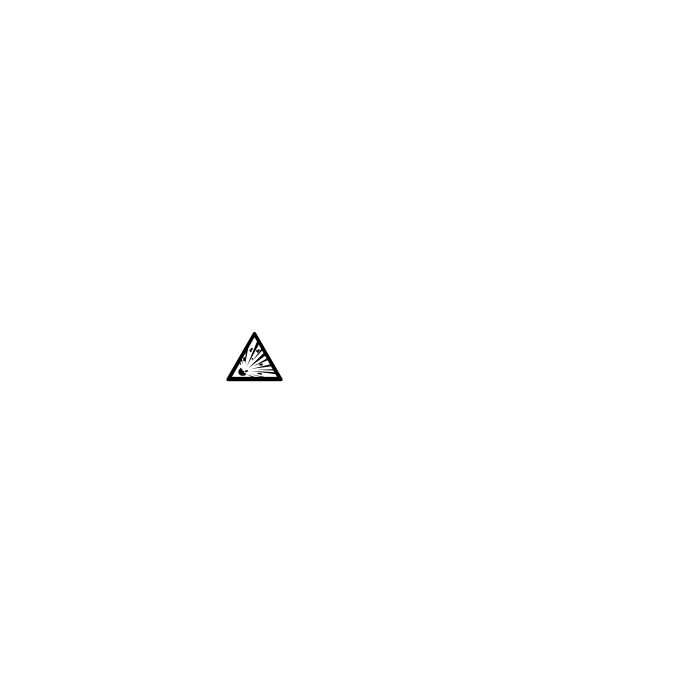
\includegraphics[height=7mm]{base/MDanger}}}\xspace}%
\newcommand{\MAttention}{\marginpar{\raisebox{-2mm}{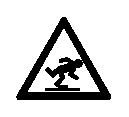
\includegraphics[height=7mm]{base/MAttention}}}\xspace}%
\newcommand{\MHint}{\marginpar{\raisebox{-2.25mm}{
\includegraphics[height=7mm]{base/MHint}}}\xspace}%
\newcommand{\MQuestion}{\marginpar{\raisebox{-2.25mm}{
\includegraphics[height=7mm]{base/MQuestion}}}\xspace}%

% same footnote number as last one
\newcommand{\oldfootnotemark}[1]{\addtocounter{footnote}{-#1}\footnotemark\addtocounter{footnote}{#1-1}}%
%\newcommand{\lastfootnotemark}{\addtocounter{footnote}{-1}\footnotemark}%

% value-unit commands (for 457 kHz, etc)
\newcommand{\vu}[2]{\mbox{\ensuremath{#1\,\text{#2}}}}% "value-unit" ... prevents e.g. 456 \linebreak mV
\newcommand{\vuc}[3]{\mbox{\ensuremath{#1\,\text{#2}\;#3\,\%}}} % "value~unit~tolerance-per-cent"
\newcommand{\vum}[3]{\mbox{\ensuremath{#1\,\text{#2}\;#3\,\perthousand}}} % "value~unit~tolerance-per-mil"

% reminders
\newcommand{\reminder}[1]{\colorbox{red}{#1}\xspace}%
\newcommand{\rem}{\reminder{(...)}}% shortcut for the full reminder
\newcommand{\remq}{\reminder{???}}% open question
\newcommand{\remc}{\reminder{[?]}}% open citation
\newcommand{\uc}{\nxtpar\colorbox{yellow}{... under construction ...}\nxtpar}%

% misc
\newcommand{\pwd}{.} % present working directory (can be used to create relativ paths per part, etc.)




% **************************************************************************************************
% * MATH
% **************************************************************************************************

% highlighting
\newcommand{\vm}[1]{\ensuremath{\bm{#1}}}% vector or matrix

% functions
\renewcommand{\exp}[1]{\ensuremath{\text{e}^{#1}}}% exponential
\renewcommand{\ln}[1]{\ensuremath{\text{ln}\!\left(#1\right)}}% natural logarithm
\newcommand{\ld}[1]{\ensuremath{\text{ld}\!\left(#1\right)}}% logarithm base 2
\renewcommand{\log}[1]{\ensuremath{\text{log}\!\left(#1\right)}}% logarithm (base 10)
\newcommand{\logb}[2]{\ensuremath{\text{log}_{#1}\!\left(#2\right)}}% logarithm base ...

% rounding
\newcommand{\round}[1]{\ensuremath{\text{round}\!\left(#1\right)}}% rounding towards next integer
\newcommand{\ceil}[1]{\ensuremath{\left\lceil#1\right\rceil}}% rounding towards infinity
\newcommand{\floor}[1]{\ensuremath{\left\lfloor#1\right\rfloor}}% rounding towards zero

% operators
\newcommand{\E}[1]{\ensuremath{\text{E}\!\left\{#1\right\}}}% expectation operator
\newcommand{\F}[1]{\ensuremath{\mathcal{F}\!\left\{#1\right\}}}% Fourier transform operator
\newcommand{\IF}[1]{\ensuremath{\mathcal{F}^{-1}\!\left\{#1\right\}}}% inverse Fourier transform operator
\newcommand{\var}[1]{\ensuremath{\text{var}\!\left\{#1\right\}}}% variance operator
\newcommand{\cov}[1]{\ensuremath{\text{cov}\!\left\{#1\right\}}}% covariance operator
\newcommand{\corr}[1]{\ensuremath{\text{corr}\!\left\{#1\right\}}}% correlation operator
\newcommand{\avg}[1]{\ensuremath{\text{avg}\!\left\{#1\right\}}}% averaging operator
\newcommand{\avgvar}[1]{\ensuremath{\overline{\text{var}}\!\left\{#1\right\}}}% average variance operator
\renewcommand{\Re}[1]{\ensuremath{\text{Re}\!\left\{#1\right\}}}% real part
\renewcommand{\Im}[1]{\ensuremath{\text{Im}\!\left\{#1\right\}}}% imaginary part

% numbers
\newcommand{\REAL}{\ensuremath{\mathbb{R}}}% real numbers
\newcommand{\NATURAL}{\ensuremath{\mathbb{N}}}% natural numbers
\newcommand{\INTEGER}{\ensuremath{\mathbb{Z}}}% integer numbers (natural numbers plus zero)
\newcommand{\COMPLEX}{\ensuremath{\mathbb{C}}}% complex numbers
\newcommand{\IMAG}{\ensuremath{\mathbb{I}}}% imaginary numbers

% other
\newcommand{\conj}{\ensuremath{^\ast}}% conjugate complex
\newcommand{\transp}{\ensuremath{^\text{T}}}% conjugate (Hermitian) transpose
\newcommand{\mtx}[2]{\left[\ensuremath{\begin{array}{#1}#2\end{array}\right]}}%vector/matrix
\newcommand{\isdef}{\ensuremath{\mathrel{:=}}}% definition left->right
\newcommand{\isdefflip}{\ensuremath{\mathrel{=:}}}% definition right->left
\newcommand{\isreq}{\ensuremath{\mathrel{\stackrel{!}{=}}}}% is required
\newcommand{\textrel}[1]{\ensuremath{{\;{#1}\;}}}% relation symbol for in-line equations (fixed spacing)



% **************************************************************************************************
% * FLOATS (FIGURES, TABLES, LISTINGS, ...)
% **************************************************************************************************

% figures without frames
%   standard
\newcommand{\fig}[3]{\begin{figure}\centering\includegraphics[width=\textwidth]{#1}\caption{#2}\label{fig:#3}\end{figure}}%
%   with controllable parameters
\newcommand{\figc}[4]{\begin{figure}\centering\includegraphics[#1]{#2}\caption{#3}\label{fig:#4}\end{figure}}%
%   two subfigures
\newcommand{\twofig}[6]{\begin{figure}\centering%
\subfigure[#2]{\includegraphics[width=0.495\textwidth]{#1}}%
\subfigure[#4]{\includegraphics[width=0.495\textwidth]{#3}}%
\caption{#5}\label{fig:#6}\end{figure}}%
%   two subfigures with labels for each subplot
\newcommand{\twofigs}[8]{\begin{figure}\centering%
\subfigure[#2]{\includegraphics[width=0.495\textwidth]{#1}\label{fig:#8#3}}%
\subfigure[#5]{\includegraphics[width=0.495\textwidth]{#4}\label{fig:#8#6}}%
\caption{#7}\label{fig:#8}\end{figure}}%
%   two subfigures and controllable parameters
\newcommand{\twofigc}[8]{\begin{figure}\centering%
\subfigure[#3]{\includegraphics[#1]{#2}}%
\subfigure[#6]{\includegraphics[#4]{#5}}%
\caption{#7}\label{fig:#8}\end{figure}}%

% framed figures
%   standard
\newcommand{\figf}[3]{\begin{figure}\centering\fbox{\includegraphics[width=\textwidth]{#1}}\caption{#2}\label{fig:#3}\end{figure}}%
%   with controllable parameters
\newcommand{\figcf}[4]{\begin{figure}\centering\fbox{\includegraphics[#1]{#2}}\caption{#3}\label{fig:#4}\end{figure}}%
%   two subfigures
\newcommand{\twofigf}[6]{\begin{figure}\centering%
\fbox{\subfigure[#2]{\includegraphics[width=0.495\textwidth]{#1}}}%
\fbox{\subfigure[#4]{\includegraphics[width=0.495\textwidth]{#3}}}%
\caption{#5}\label{fig:#6}\end{figure}}%
%   two subfigures with labels for each subplot
\newcommand{\twofigsf}[8]{\begin{figure}\centering%
\fbox{\subfigure[#2]{\includegraphics[width=0.495\textwidth]{#1}\label{fig:#8#3}}}%
\fbox{\subfigure[#5]{\includegraphics[width=0.495\textwidth]{#4}\label{fig:#8#6}}}%
\caption{#7}\label{fig:#8}\end{figure}}%
%   two subfigures and controllable parameters
\newcommand{\twofigcf}[8]{\begin{figure}\centering%
\fbox{\subfigure[#3]{\includegraphics[#1]{#2}}}%
\fbox{\subfigure[#6]{\includegraphics[#4]{#5}}}%
\caption{#7}\label{fig:#8}\end{figure}}%

% listings
\newcommand{\filelisting}[4]{\lstinputlisting[print=true,language=#1,caption={#3},label={lst:#4}]{#2}}

% preserve backslash for linebreaks in tables (ragged... redefines \\, thus it has to be preserved)
\newcommand{\pbs}[1]{\let\temp=\\#1\let\\=\temp}%


% **************************************************************************************************
% * MISC
% **************************************************************************************************

% slighly darkened colors for text
\definecolor{bkred}{rgb}{0.9,0,0}
\definecolor{bkgreen}{rgb}{0,0.67,0}
\definecolor{bkblue}{rgb}{0,0,0.75}